
\chapter{Grundlagen }

In diesem Kapitel werden Grundbegriffe und Zusammenhänge der Kompression, Approximation und insbesondere der LZ-Zerlegung erläutert.
\section{Zahlen}
Im Laufe de Arbeit steht $PRIME$ für die Menge der Primzahlen. Eine Zahl $x$ ist eine Primzahl wenn die einzigen beiden Teiler von $x$ die Zahl $1$ und $x$ selber sind. Eine Zahl $n$ steht für eine beliebige natürliche Zahl $n\in\mathbb{N}$.

\section{Kompression}

\emph{Kompression} ist die Transformation von Daten in eine kleinere Darstellung.
Es gibt zwei Möglichkeiten diese Transformation auszuführen, verlustfrei oder verlustbehaftet.
Alle verlustfreien Ansätze basieren darauf, Redundanzen innerhalb eines Datensatzes zu eliminieren, während verlustbehaftete Methoden ausgewählte Daten löschen.
Der bedeutende Unterschied zwischen diesen beiden Ansätzen ist, dass sich nur aus einer verlustfreien Kompression das Original wiederherstellen lässt.\\
Die Güte einer Kompression, der \emph{Kompressionsgrad}, ist definiert als:
\begin{equation}\nonumber
\text{Kompressionsgrad} =\frac{\text{Gr"o\ss e der Ausgabe}}{\text{Gr"o\ss e der Eingabe}}
\end{equation}
\\
\noindent
Während der \emph{Kompressionsfaktor} das Inverse des Kompressionsgrades ist:
\begin{equation}\nonumber
\text{Kompressionsfaktor} =\frac{\text{Gr"o\ss e der Eingabe}}{\text{Gr"o\ss e der Ausgabe}}
\end{equation}
\\
\noindent
Keine verlustfreie Kompressionsmethode kann einen Kompressionsgrad $<1$ garantieren, ein Kompressionsgrad ist immer von der Eingabe abhängig. Sollte theoretisch eine solche Methode existieren, könnte man sie immer wieder auf ihre eigenen Ausgaben anwenden und jegliche Datenmenge in nur einem einzelnen Bit codieren, was offensichtlich unmöglich ist \cite{compressreff}.\\
In dieser Arbeit beschäftige ich mich ausschließlich mit verlustfreien Verfahren, der Begriff der Kompression bezieht sich deshalb immer auf die verlustfreie Kompression.


\section{Strings}
Eine fundamentale Art Informationen darzustellen ist der \emph{String}.
Ein \emph{String} $w$ der Länge $n$ ist eine Folge von Symbolen $w[1],w[2],\cdots ,w[n-1]$ aus einem Alphabet $\Sigma$.\\
Ein String $u$ der Länge $m$ ist Substring von $w$, wenn für ein $i<n-m$ gilt:

$u[1]u[2] \cdots u[m-1] = w[i]w[i+1] \cdots w[m-1]$.\\
Der Substring  $u$ besitzt einen \emph{vorherigen Substring} in $w$, wenn ein $x<i$ existiert mit:

$w[i+0]w[i+1] \cdots w[m-1] = w[x+0]w[x+1] \cdots w[x-1]$.\\
Der folgende/nächste Substring von $w[i,j]$ ist $u[i+1,j+1]$.\\
Für Substrings  existieren zwei Kategorien mit besonderer Bedeutung, Präfixe und Suffixe.
Präfixe sind Substrings, die an Index $1$ beginnen, während Suffixe Substrings  sind, die an Index $n$ enden.
Als \emph{echte Substrings}  bezeichnet man Substrings  die kürzer sind als der String  in dem sie liegen.
Im Folgenden soll \emph{Substring}[$i,j$] den Substring  der an Index \textit{i} beginnt und an Index \textit{j} endet bezeichnen.\\
In \textit{C++} existieren zwei Konzepte, die als String  bezeichnet werden, der \textit{C-style char array} und die \textit{std::string} Klasse.
Das \textit{C-style char array} ist ein kontinuierlicher Block an Speicher mit fester Größe. In diesem Block liegen \textit{chars}, die Symbole darstellen, direkt hintereinander. Die Größe des \textit{arrays} kann nachträglich nicht verändert werden.\\
Die \textit{std::string} Klasse spezifiziert Objekte, die ein \textit{char array} enthalten. Objekte der Klasse String  bieten weitere Funktionalitäten und die Möglichkeit, die Länge des Strings  zu verändern \cite{cplusplus}.

\section{LZ-Zerlegung}
Eine LZ-Zerlegung ist eine Aufteilung eines String \textit{T} in sich nicht überschneidende Substrings, diese Substrings  bezeichnet man als Faktoren.
Das heißt für jeden Faktor $f[i,j]$, also jeden Substring$[i,j]$ in der LZ-Zerlegung $LZ()$ der Eingabe $T$ gilt:
\begin{itemize}
	\item Die Faktoren überschneiden sich nicht: $T = f_1  f_2 f_3 \cdots f_n$
	\item Die Faktoren sind einzelne Symbole oder besitzen vorherige Substrings
	\item Die Faktoren sind in ihrer möglichen Länge maximal, d.h. keine zwei aufeinander folgenden Faktoren können zusammen ein Faktor sein
	
\end{itemize}
Die LZ-Zerlegung erlaubt es einen String  komprimiert darzustellen.
Diese Kompression wird erreicht, indem in der LZ-Zerlegung Faktoren durch Referenzen ersetzt werden.
Jede Referenz ist ein Tupel aus zwei Zahlen, das  einen vorher liegenden Substring  identifiziert.
Das erste Element des Tupels enthält Informationen über die Position des vorher liegenden Substrings, während das zweite Element die Länge des Substrings angibt.
Die Positionsangabe kann dabei ein \textit{offset} oder ein absoluter Index über den faktorisierten  String  sein.
Ein \textit{offset} ist meist aber kleiner, da für größere Strings  ein absoluter Index $\lceil \log_2{n}\rceil$ Bits belegt (wobei $n = |T|$), wohingegen ein offset nur im \textit{worst case} genau so groß ist.\\
Allerdings werden nicht alle Substrings  durch Referenzen ersetzt.
Wenn die zugehörige Referenz mehr Speicher benötigt als der Faktor selbst, lohnt es sich nicht den Substring  zu ersetzten.
Deshalb wird auch keine Referenz gespeichert, wenn der Faktor ein einzelnes Symbol ist \cite{LZ77}.


\section{Approximation}

Zu jedem Optimierungsproblem existiert eine Menge an richtigen Lösungen und in dieser eine Teilmenge an optimale Lösungen. 
Ein Approximationsalgorithmus erzeugt für eine Eingabe eine richtige Lösung, die aber nicht zwangsläufig optimal sein muss.\\
Die \emph{Approximationsgüte} $\rho$ ist eine Garantie, wie sehr die erzeugte Lösung \textit{s\textsubscript{e}} maximal von einer optimalen Lösung \textit{s\textsubscript{opt}} abweicht. Um nichtnumerische Ergebnisse vergleichen zu können, evaluiert man beide durch eine Bewertungsfunktion \textit{f(s)} \cite{approxdef}. Dann ist 
\begin{equation}\nonumber
\rho= max
\left\{
\frac{f(s_{e})}{f(s_{opt})},\frac{f(s_{opt})}{f(s_{e})}
\right\}
\end{equation}
Da eine Abweichung vom Optimum sowohl größer als auch kleiner als eins sein kann, ist der größere der beiden Brüche die Güte.

\section{LZ-Approximation}
Zu jedem beliebigen String  existiert genau eine LZ-Zerlegung. Eine Approximation dieser Zerlegung besteht, wenn die Faktoren in ihrer Länge nicht zwingend maximal sind. Die Faktoren der Approximation sind weiterhin entweder einzelne Symbole oder besitzen vorherige Substrings.\\
Eine \textit{c-optimalen} \emph{Approximation} besteht dann, wenn keine \textit{c} aufeinander folgenden Faktoren selber einen Faktor bilden. 
Daraus folgt, dass in einem Faktor der LZ-Zerlegung maximal c-1 ganze Faktoren liegen können. Es kann aber sein, dass sowohl ein echtes Suffix und ein echtes Präfix der umliegenden Faktoren ebenfalls in dem Faktor der LZ-Zerlegung enthalten sind. Im ungünstigsten Fall wird damit ein Faktor vollkommen zwischen zwei Faktoren der LZ-Zerlegung aufgeteilt (vgl. Abb. \ref{flz}). 
%
\begin{figure}[h]
	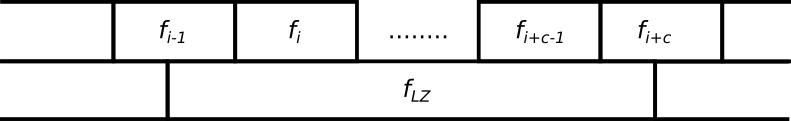
\includegraphics[width=\textwidth,keepaspectratio]{faktorenmerge}
	\caption{Der Faktor $f_{LZ}$ erstreckt sich von $f_{i-1}$ bis $f_{i+c}$}
	\label{flz}
\end{figure}\\
Das bedeutet, dass wir maximal $c$-mal mehr Faktoren in der \textit{c-optimale} LZ-Approximation finden als in der  LZ-Zerlegung.
Die Anzahl der Faktoren in der Approximation ist also durch die Anzahl der Faktoren in der LZ-Zerlegung multipliziert mit $c$ nach oben beschränkt.  
\begin{equation}\nonumber
\rho = max
\left\{
\frac{c*f(s_{opt})}{f(s_{opt})},\frac{f(s_{opt})}{c * f(s_{opt})}
\right\} = c
\end{equation}
Aus einer \textit{c-Optimalität} der Approximation folgt eine Güte der Approximation von $c$ \cite{LZ77Approx}.\\

\section{Hashfunktionen}

Eine \emph{Hashfunktion} $h$ ist eine Funktion von einem \emph{Universum U} auf eine beschränkte Teilmenge der natürlichen Zahlen $h:U \rightarrow \{0,1,2\cdots ,n \}$.
Die Ausgaben bezeichnet man als Schlüssel oder auch als \emph{Hashwert/Hashcode}, eine Hashfunktion definiert damit \emph{key value pairs}.
Wenn unterschiedliche Werte den gleichen Hashcode besitzen, bezeichnet man dies als \emph{Kollision}.
Wenn die Menge der Eingaben größer ist als die Menge der Hashcodes sind Kollisionen unvermeidlich.\\
Eine Hashfunktion wird anhand folgender zentraler Kriterien bewertet:
\begin{itemize}
	\item Verteilung: Alle möglichen Hashwerte sollen gleich wahrscheinlich getroffen werden
	\item Dichte: Die Menge aller Hashwerte soll möglichst klein sein
	\item Kollisionswahrscheinlichkeit: Kollisionen sollen möglichst gering sein
\end{itemize}
Diese Güten einer Hashfunktion müssen allerdings im Hinblick auf die Eingabewerte betrachtet werden. Für Eingabemengen mit sehr kleinem Alphabet z.B. DNA mit \{G,A,T,C\} können Funktionen gut funktionieren, die für Alphabete mit z.B. allen möglichen Werten pro Byte sehr oft zu Kollisionen führen\cite{joyhash}.\\

\section{Hashmaps}

\noindent
Die \emph{Hashmap} ist eine Datenstruktur die $Lookups$, das Einfügen und das Löschen in erwartet konstanter Zeit ermöglicht. Dies ist einer der häufigsten Anwendungsfälle der  Hash\-funktionen.
Beim Einfügen eines Elementes $e$ wird der Hashwert von $e$, $h(e)$, berechnet und $e$ unter Index $h(e)$ abgespeichert, dabei kann es hier zu einer Kollision kommen.
Um zu überprüfen, ob ein Element $e$ in der Hashmap enthalten ist, genügt es den Hashwert zu berechnen und nur den so erhaltenen Index zu untersuchen.
Das Löschen eines Elementes verläuft ebenso, außer dass nach dem Auffinden das entsprechende Element gelöscht wird.\\
Ein Speicherplatz in einer Hashmap bezeichnet man auch als \emph{Bucket}.

\noindent
Um mit Kollisionen effizient umzugehen existieren zahlreiche Ansätze, zu den bekanntesten zählen:
\begin{itemize}
	\item \emph{chaining}: die verschiedenen Elemente einfach in einer Liste zu verketten
	\item  \emph{double hashing}: hinter jedem Index eine zweite Hashmap zu bilden
	\item \emph{linear probing}: das  Element unter dem nächsten freien Index zu speichern
	\item \emph{quadratic probing}: das Element unter dem doppelten Index zu speichern
\end{itemize}
Alle Kollisionsresolutionsmethoden haben ihre eigenen Vor- und Nachteile \cite{joyhash}\cite{datastructguide}.


\section{Fingerprint}
Als \textit{Rabin-Karp-Fingerprint}, im Folgenden einfach Fingerprint, bezeichnet man den Hashcode eines Strings.
Fingerprints erlauben es, Strings schneller zu vergleichen.
Um herauszufinden ob zwei Strings $s_{1}, s_{2}$ gleich sind müssen wir alle Symbole miteinander vergleichen.
Sollten die beiden Strings sich nur im letzten Symbol unterscheiden, so haben wir alle vorherigen Symbole umsonst überprüft.\\
Vergleichen wir aber vorher beide Fingerprints können wir ungleiche Strings direkt daran erkennen. Dies ist wesentlich effizienter, da Fingerprints meist deutlich kürzer sind als die Strings selber.
Es kann aber sein, dass durch eine Kollision unterschiedliche Strings den gleichen \textit{Fingerprint} besitzen.
Daher reicht es nicht aus, nur die Fingerprints zu vergleichen.
Wenn  zwei Fingerprints gleich sind, müssen danach alle Symbole der Strings untersucht werden\cite{Karp1987}\cite{joyhash}.

\section{rolling Hash}
Ein \textit{rolling Hash} ist eine rekursive Methode, um aus dem Fingerprint eines Substrings $w$ den Fingerprint des nachfolgenden Substrings $u$ zu erhalten.\\
Wenn wir einen Text $T$ durchsuchen, müssen wir für jede Position den Hashwert des Substrings bilden. Da die benötigte Zeit um einen Fingerprint zu berechnen von der Länge des Substrings abhängt, kann dies für lange Substrings zeitintensiv sein. Ein rolling Hash beschleunigt die Berechnung von Hashwerten aufeinander folgender Substrings, indem er ausnutzt, dass sich die Substrings nur in zwei chars unterscheiden. In einem rolling Hash entfernen wir sozusagen den nicht mehr vorhandenen char aus dem Hashwert und fügen den neuen char hinzu \cite{Karp1987}.\\
Allerdings eignen sich nicht alle Hashmethoden für einen rolling Hash. Um einen rolling Hash zu ermöglichen, muss die Hashfunktion folgende Eigenschaften aufweisen:
\begin{equation}\nonumber
	h(u)=h(w)-f(w_{0})+f(u_{m})
\end{equation}
\noindent
Wobei $m$ die Länge der Substrings und $f()$ die Transformation der einzelnen $chars$ ist. Diese Eigenschaft erfüllen nicht alle Hashfunktionen. Im Pearson Hash wird aus einem String lediglich ein Index für eine Substitutionstabelle berechnet, die die eigentlichen Hash\-werte enthält \cite{pearsonhash}. Da diese Substitution nicht rückführbar ist, ohne die ganze Tabelle zu durchsuchen, eignet sich diese Hashfunktion nicht als rolling Hash.\\

\subsection{Polynomen Hash}

Ein \textit{Polynom Hash} ist eine intuitive Methode, um den Fingerprint eines Strings zu berechnen. 
Ein Polynomen Hash besteht aus drei Parametern:
\begin{itemize}
	\item eine Funktion die jedem Symbol des Eingabealphabetes einen numerischen Wert zuordnet $f()$
	\item  eine Primzahl $p$ als Potenzbasis 
	\item die Länge der zu hashenden Strings $l$
\end{itemize} 
Der Hashwert eines Strings $w$ wird wie folgt berechnet:
\begin{equation}\nonumber
Hash(w)=\sum_{0}^{l}f(w[i])*p^{l-i}
\end{equation}
\noindent
So lässt sich der Fingerprint des nächsten Substrings $u$ wie folgt aus dem Fingerprint des aktuellen Substrings $w$ berechnen:
\begin{equation}\nonumber
	Hash(u)=Hash(w)-f(w[0])*p^{l}+f(u[l])
\end{equation}
Da bei langen Substrings \textit{Overflows} (wir erhalten eine Zahl die nicht in unsere Bitdarstellung passt) auftreten können, wenden wir nach jedem Berechnungsschritt eine Modulofunktion an. Zur Vermeidung von Kollisionen ist die Zahl mit der wir Modulo rechnen meist auch eine Primzahl $p_m \in PRIME$ \cite{joyhash}\cite{Karp1987}.
\begin{equation}\nonumber
	Hash(w)=\sum_{0}^{l}(f(w[i])*p^{l-i})\%p_m	
\end{equation}
Man muss ebenfalls beachten, dass die Primzahl mit der Länge als Exponent keinen Overflow verursacht.  Diesen \textit{Exponentenwert} berechnen wir daher wie folgt:
\begin{align}\nonumber
	exp_0&=p\\ \nonumber
	exp_n&= (exp_{n-1} \% p_m ) * p
\end{align}
Die Berechnung endet wenn $n=l$ ist.

\subsubsection{Wahl der Primzahlen}

Die Wahl geeigneter Primzahlen ist für einen Polynomen Hash sehr wichtig. Sie haben Einfluss auf die Wahrscheinlichkeit einer Kollision und die Streuung der Hashwerte über den Wertebereich. Folgende Grundregeln sind bei der Wahl der Primzahlen zu beachten:
\begin{itemize}
	\item  sei $p$ eine Primzahl die größer ist als  der maximale Wert von $f()$
	\item die Primzahl mit der man Modulo rechnet $p_m$ sollte so groß wie möglich sein
	\item  sei $l$ die Länge der Strings, dann soll gelten dass $p^l *max(f())$ keinen Overflow verursachen
\end{itemize}
\cite{joyhash}\cite{LZ77Approx}

\subsubsection{Mersenne und Fermat Primzahlen}


Mersenne Primzahlen sind Primzahlen die genau eins weniger sind als eine Zweierpotenz
\begin{equation}\nonumber
	p \in MERSENNEPRIME. p \in PRIME \land p= 2^n -1 \land n \in \mathbb{N} 
\end{equation} 
Mit diesen Zahlen lässt sich die relativ rechenzeitintensive Modulooperation vereinfachen.
\begin{equation}\nonumber
	z \text{ mod } p =
	\begin{cases}\!%
			(z\&p)+(z>>n)-p, p<(z\&p)+(z>>n) \nonumber \\
			(z\&p)+(z>>n) , p\leq(z\&p)+(z>>n) \nonumber
	\end{cases}
\end{equation}
\noindent
Dieses Vorgehen kann schneller sein da keine Division ausgeführt werden muss.\\
Fermat Primzahlen können besonders schnell multipliziert werden.  Fermat Primzahlen sind immer genau eins mehr als eine Zweierpotenz. Daher gilt:
\begin{align}\nonumber
	&x\in FERMATPRIME,y\in\mathbb{N} . 2^y+1=x \\
	&s*x=(s<<y)+s  \nonumber
\end{align} 
	
\subsection{Buzhash}

Ein \emph{Buzhash} ist eine Variante des Tabellenhashens die lediglich Substitutionen, Verundung, Bitshifts und Antivalenzen anwendet. Dies macht die Berechnung besonders schnell.\\
Die Grundidee des Buzhashing ist es, den vorhandenen Hash  zu rotieren und aus der Rotation und dem neuen char die Antivalenz zu bilden.
Die $n$-te Rotation $rotatation^n(x)$  oder der $n$-te \emph{cyclic shift} von $x$:  entspricht dem $n$-fachen Tauschen aller Bits mit ihrem Vorgänger, wobei der Vorgänger des ersten Bits das letzte Bit ist. Um weniger Kollisionen zu erhalten, kann man eine Substitutionsfunktion $f()$ auf die chars anwenden \cite{buzhash}\cite{joyhash}.

\subsection{ntHash}
Der \textit{ntHash} ist eine Hashfunktion die speziell für das Alphabet der DNA \{A,C,G,T\} konzipiert wurde \cite{nthhash}.
Ein ntHash Fingerprint einer Nukleotidsequenz $w$ mit Länge $l$ wird in drei Schritten berechnet. Als erstes wird jedes Symbol durch ein 64Bit Wert ersetzt, danach rotieren wir diese Werte anhand ihrer Position in der Sequenz.
Zum Schluss bilden wir die Antivalenz aus all diesen Werten.
\begin{align} 
	&Fingerprint(w)=\nonumber \\
	& rotation^{l-1}(h(w[0]))\oplus rotation^{l-2}(h(w[1]))\oplus\cdots
	 \oplus rotation^{1}(h(w[l-1]))\oplus h(w[l])\nonumber
\end{align}
Aus einem ntHash Fingerprint eines Substrings $T[i, k]$ mit Länge $l=k-i$ von Text $T$  lässt sich leicht der Fingerprint des folgenden Substrings $T[i+1, k+1]$ berechnen.
Wir berechnen die $l$-te Rotation der Substitution des Symbols an Stelle $i$ und die Substitution des Symbols an Stelle $k+1$. Aus diesen drei bilden wir die Antivalenz:
\begin{align}
	Fingerprint(&T[i+1, k+1])= \nonumber \\ 
	&rotation^1(Fingerprint(T[i,s k]))\oplus rotation^k(h(T[i]))\oplus h(T[i+k])\nonumber
\end{align}
Diese Hashfunktion zeichnet sich dadurch aus, dass keine Addition, Multiplikation, Modulo oder Subtraktion ausgeführt werden muss und dass sie besonders wenig Kollisionen erzeugt \cite{nthhash}.